
\setbeamerfont{block title}{size=\scriptsize}
\setbeamerfont{block body}{size=\scriptsize}
\setbeamerfont{exampleblock title}{size=\scriptsize}
\setbeamerfont{exampleblock body}{size=\scriptsize}

\begin{frame}{Les systèmes de systèmes}
\centering 
%\begin{tabular}{cc}
%Dirigé & Consensuel \\
%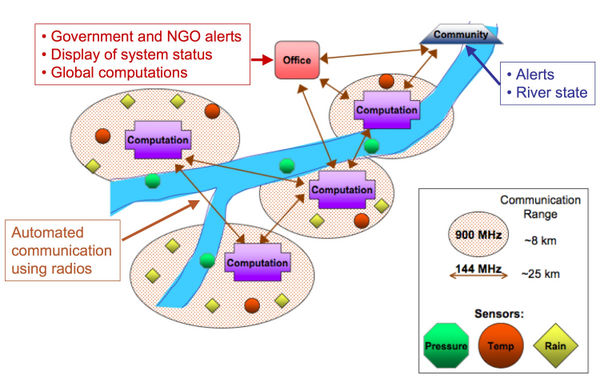
\includegraphics[width=3cm, height=2cm]{imgs/fms.jpeg} &
%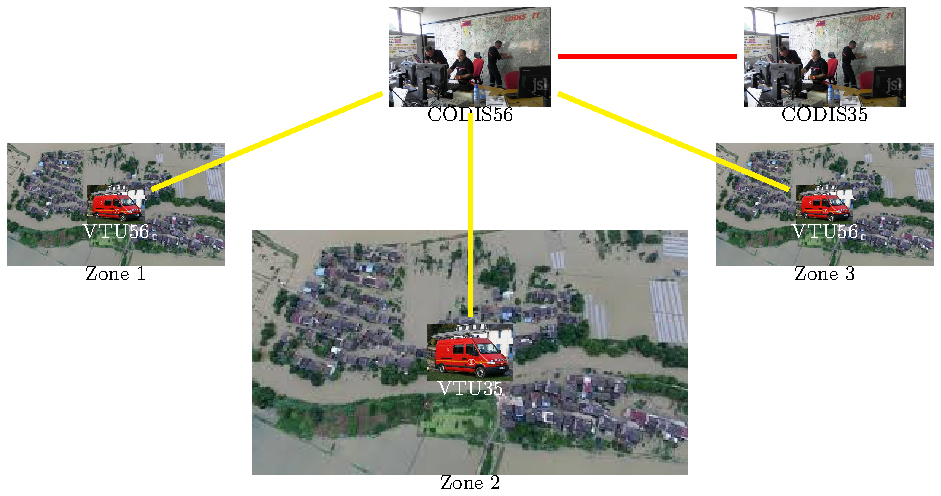
\includegraphics[width=3cm, height=2cm]{imgs/fig_overview_conf1.pdf}\\
%Surveillance d'inondation \vspace{0.2cm}& Service d'urgence\vspace{0.2cm}\\
%Collaboratif & Virtuel \\ 
%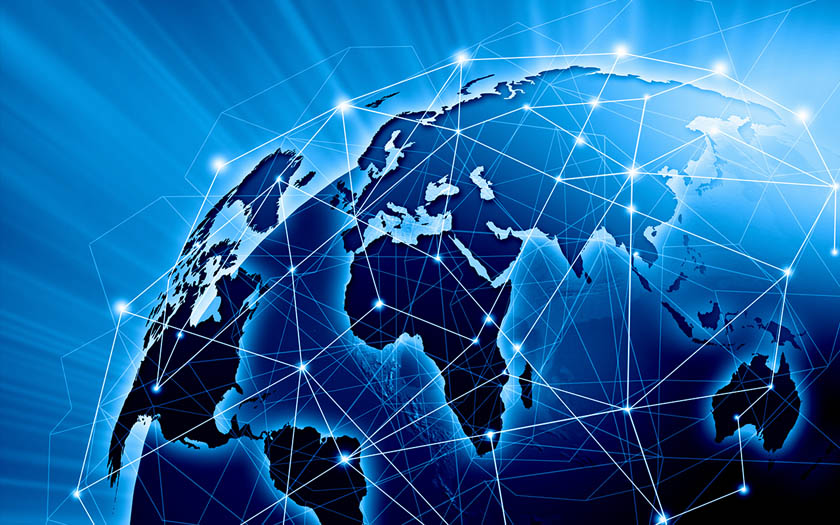
\includegraphics[width=3cm, height=2cm]{imgs/internet.jpg} &
%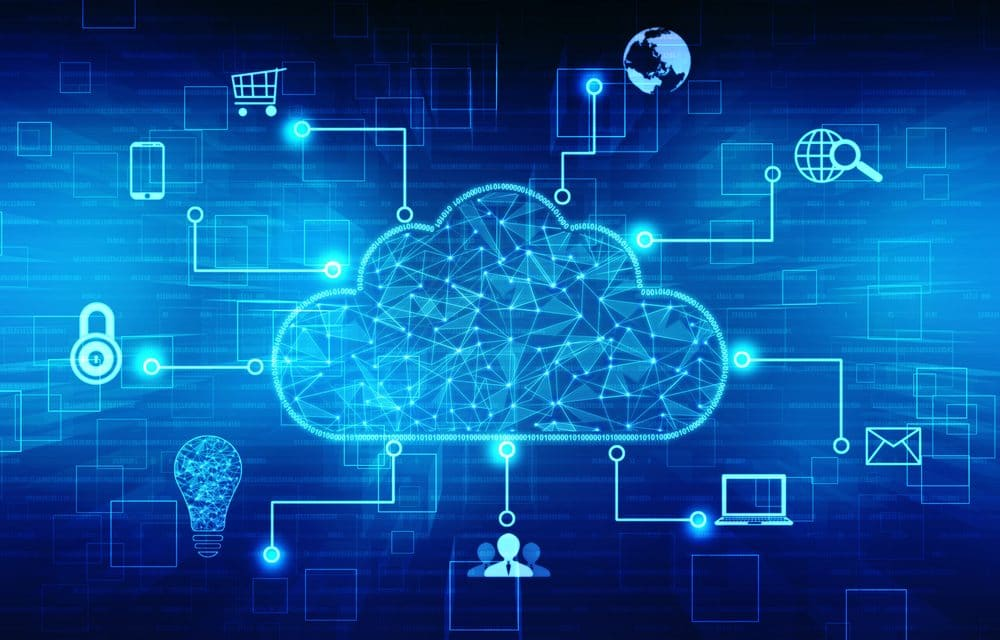
\includegraphics[width=3cm, height=2cm]{imgs/web.jpg}\\
%Internet & Web \\
%\end{tabular}
\begin{columns}
\begin{column}{0.4\textwidth}
\begin{block}{}
\begin{itemize}
\item  Ses systèmes constituants (CSs) sont \textbf{géographiquement
distribués}, 
\item possèdent leur propre \textbf{indépendance
opérationnelle} et
\textbf{managériale}. 
\item L'intéraction de ces CSs produit un \textbf{comportement
émergent}. 
\item Le SdS a un \textbf{développement évolutionnaire}.
\end{itemize} 
\end{block}
\end{column}
\begin{column}{0.5\textwidth}
\begin{figure}
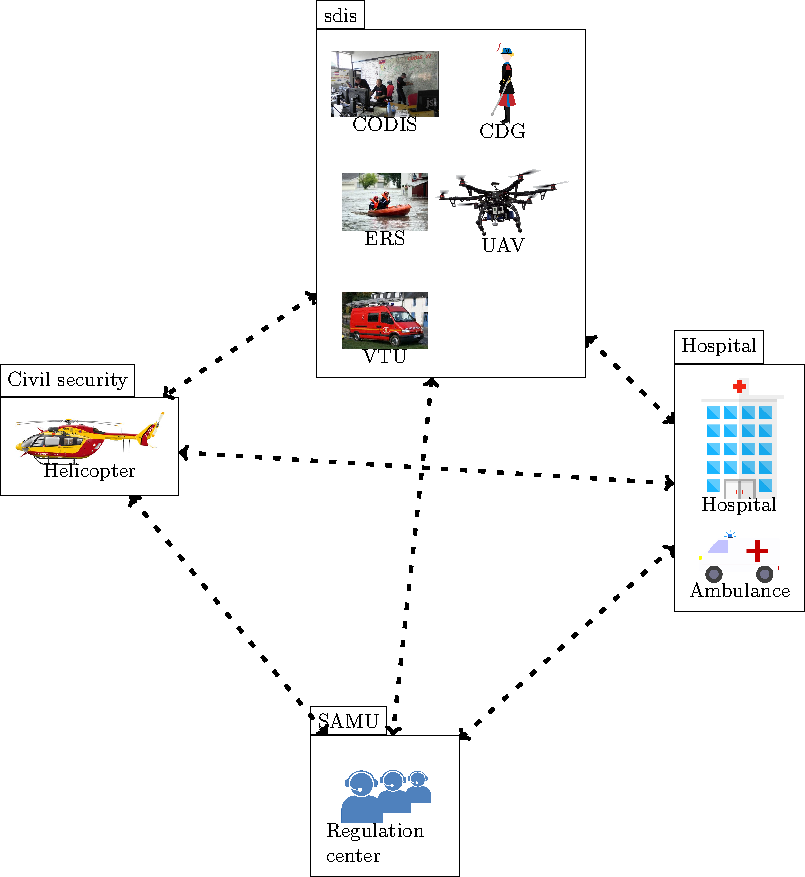
\includegraphics[height=\textwidth]{imgs/fig_sos_overview.pdf}
\caption{\underline{\textbf{Service de secours Français}}}
\end{figure}
\end{column}
\end{columns}
\end{frame}

\begin{frame}{Développement évolutionnaire}

\begin{textblock*}{4.5cm}(80mm,15mm)
\begin{block}{}
Le \textbf{développement évolutionnaire} est l'\textbf{évolution
constante} \\
des \textbf{fonctions} et \textbf{buts} du SdS.
\end{block}
\end{textblock*}

\begin{figure}
%\centering
\flushleft
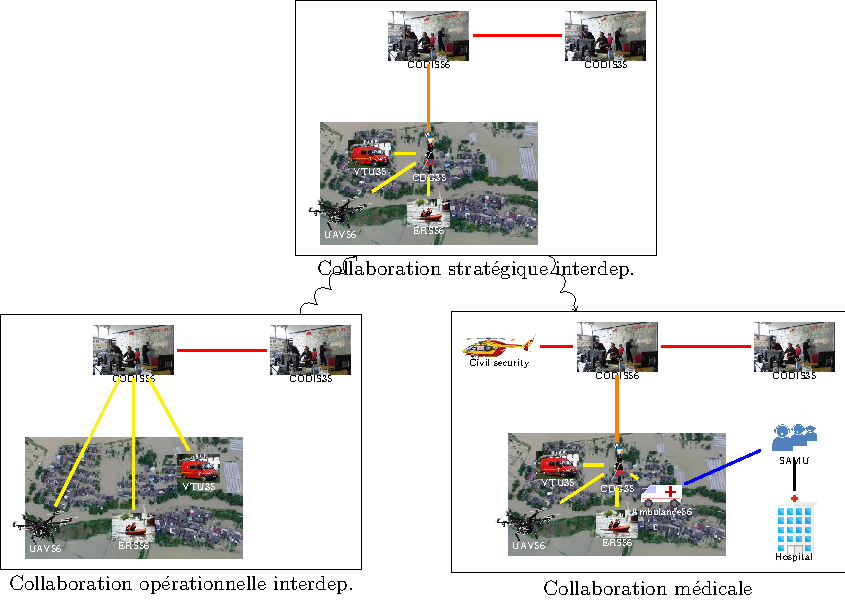
\includegraphics[width=9cm]{imgs/dev_evolutionnaire.pdf}
\end{figure}
\end{frame}


\begin{frame}{Problématique : variabilité des décisions}
\begin{block}{}
La \textbf{reconfiguration dynamique} est une phase du
développement d'un système qui consiste à le modifier pendant qu’il est
utilisé. La reconfiguration peut être corrective, fonctionnelle,  ou
non-fonctionnelle.
\end{block}
\begin{figure}
%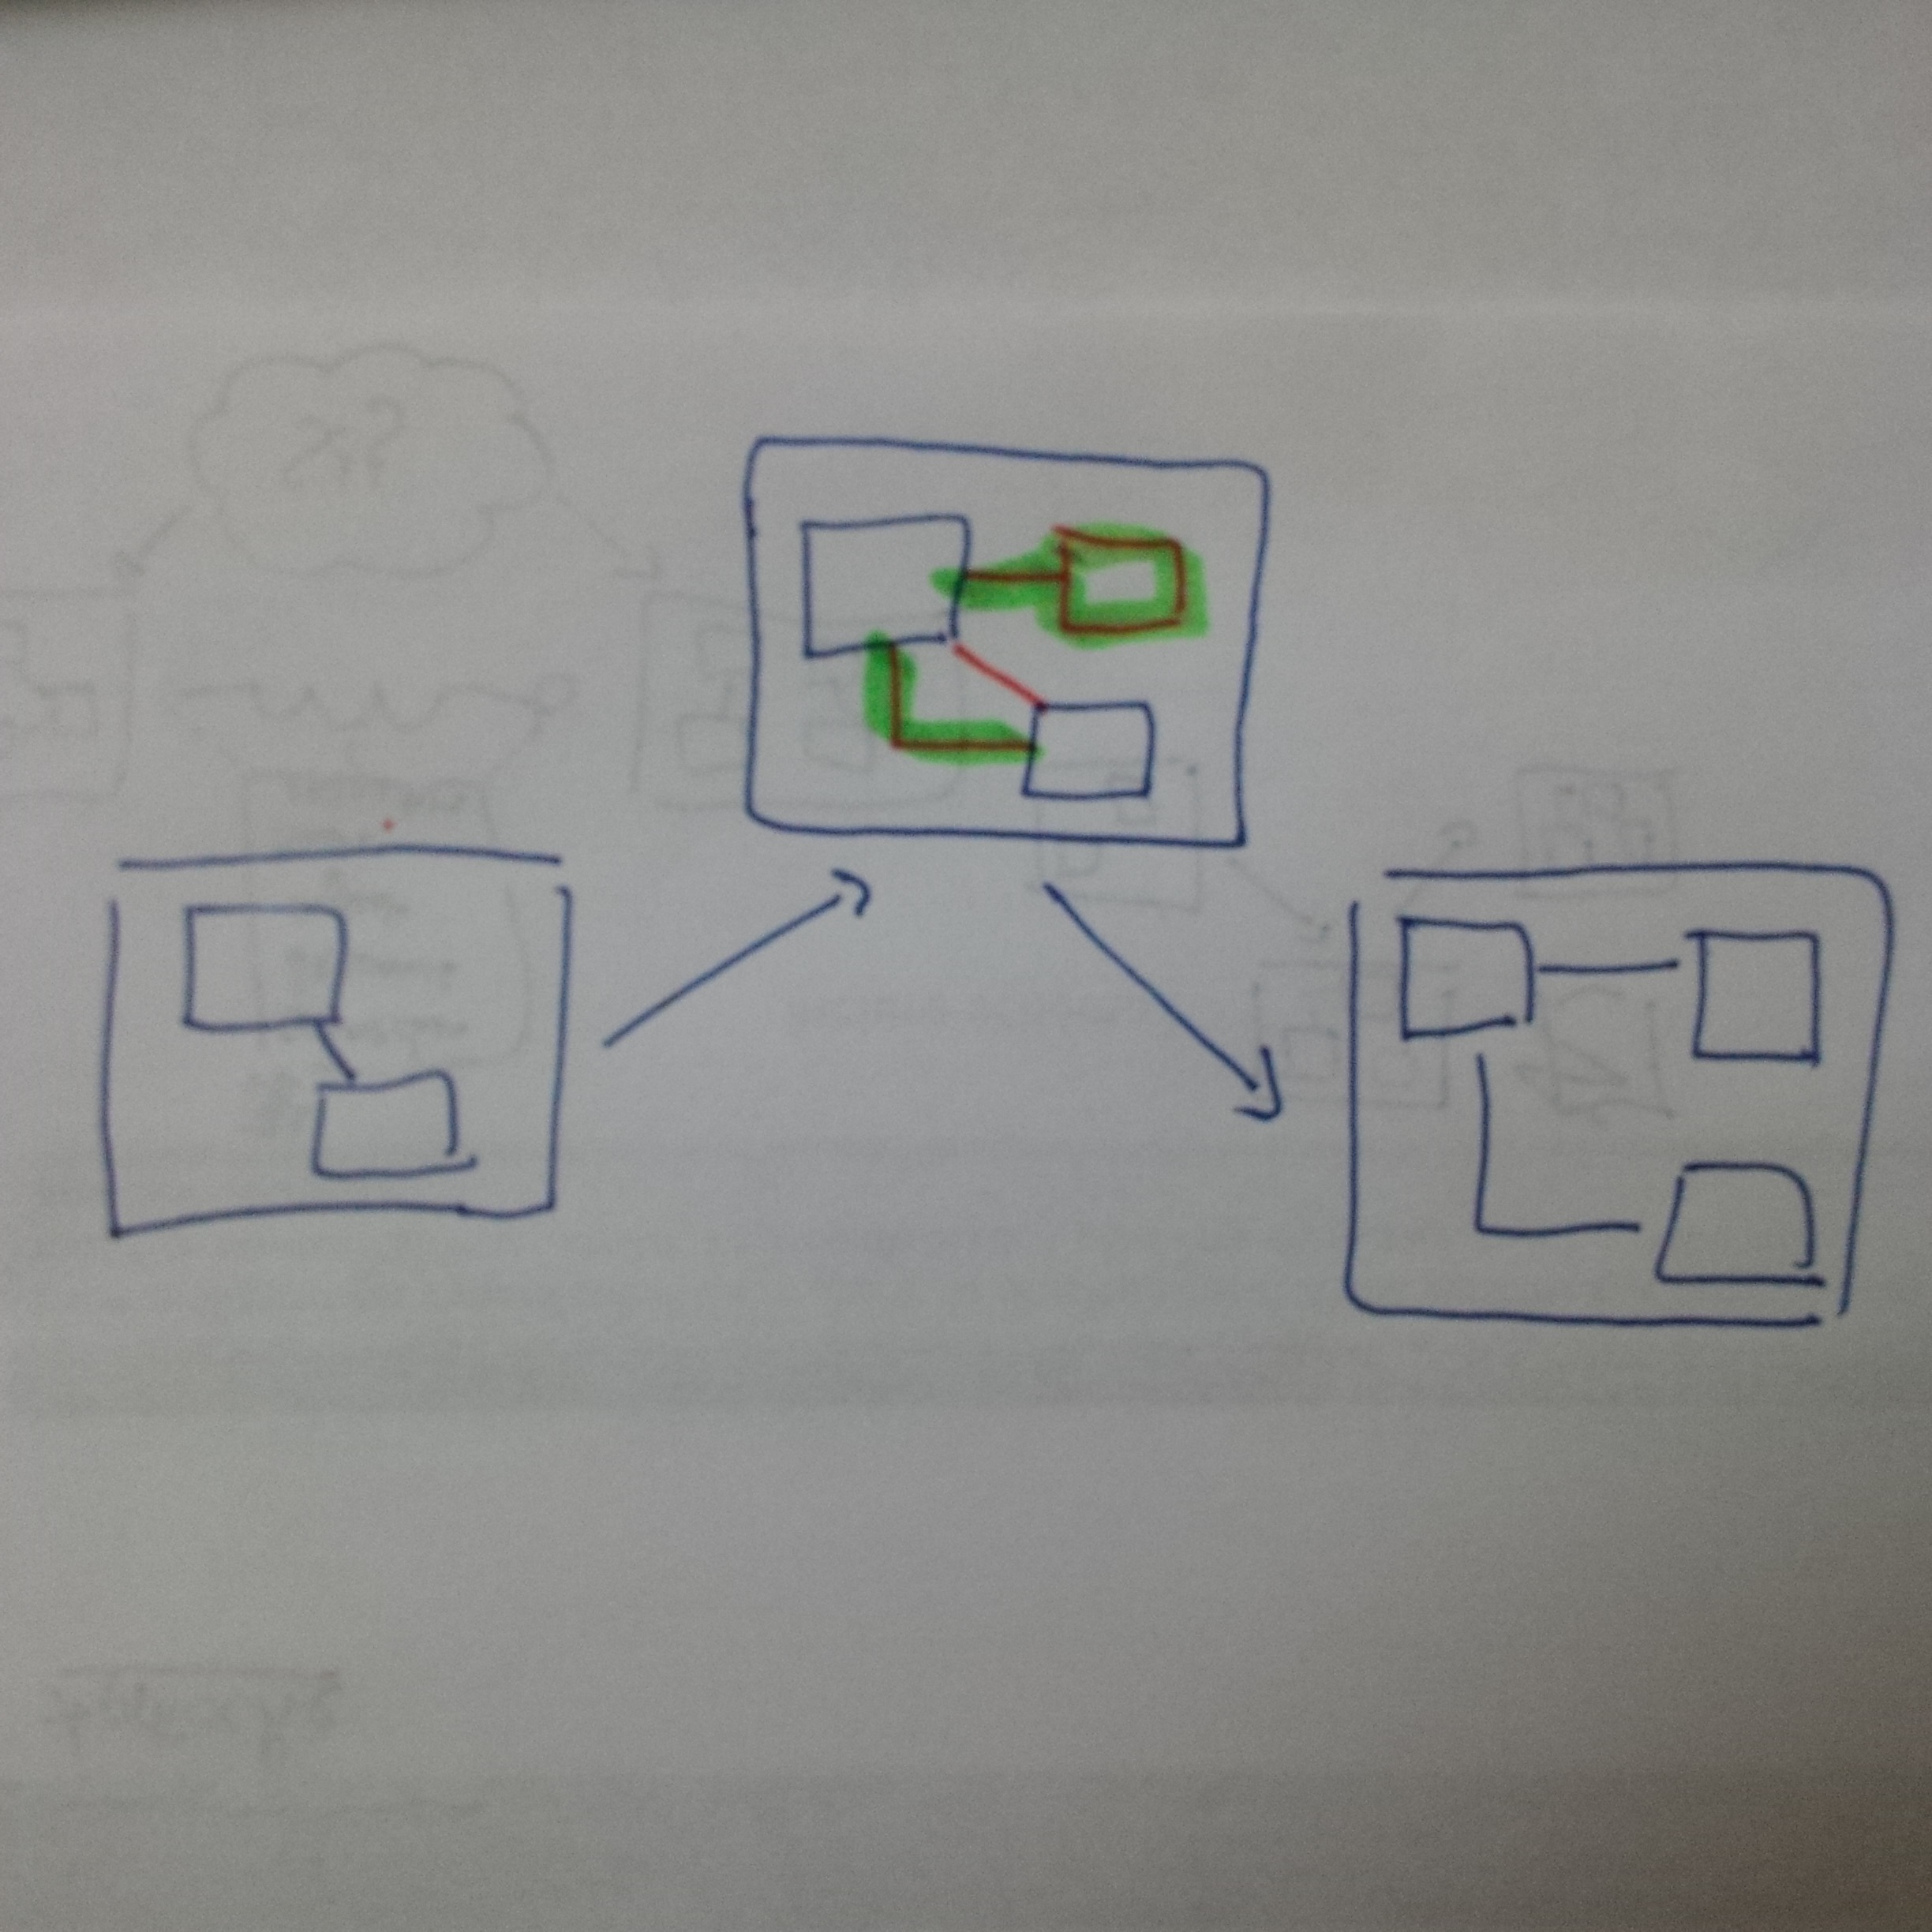
\includegraphics[height=6cm]{imgs/description_reconfiguration}
\begin{tikzpicture}
    \begin{scope}[line width=2pt]
        \begin{scope}[every node/.style={draw=black,rectangle,minimum height=5mm,minimum width=5mm,line width=2pt},node distance=2.5mm]
            \foreach \i/\xs/\ys in {0/0cm/0cm,1/3cm/9mm,12/6cm/9mm,9/3cm/-9mm,92/6cm/-9mm,2/9cm/0cm} {
                \begin{scope}[xshift=\xs,yshift=\ys]
                    \node (a\i) {};
                    \node[below right=of a\i] (b\i) {};
                \end{scope}
            }
            \foreach \i in {12,9} {
                \node[draw=green!70!black,right=of a\i] (c\i) {};
            }
            \foreach \i in {92,2} {
                \node[right=of a\i] (c\i) {};
            }
        \end{scope}
        \begin{scope}[draw=black]
            \draw (a0) -- (b0);
            \foreach \i in {92,2} {
                \draw (a\i) |- (b\i);
                \draw (a\i) -- (c\i);
            }
        \end{scope}
        \begin{scope}[draw=green!70!black]
            \foreach \i in {12,9} {
                \draw (a\i) |- (b\i);
                \draw (a\i) -- (c\i);
            }
        \end{scope}
        \foreach \i in {1,92} {
            \draw[red!70!black] (a\i) -- (b\i);
        }
    \begin{scope}[every node/.style={line width=2pt,draw,rectangle}]
        \foreach \i in {0,1} {
            \node[fit=(a\i)(b\i)] (C\i) {};
        }
        \foreach \i in {12,9,92,2} {
            \node[fit=(a\i)(b\i)(c\i)] (C\i) {};
        }
    \end{scope}
        \begin{scope}[->]
            \draw (C0) to[out=10,in=180] (C1);
            \draw (C0) to[out=350,in=180] (C9);
            \draw (C1) -- (C12);
            \draw (C9) -- (C92);
            \draw (C12) to[out=0,in=170] (C2);
            \draw (C92) to[out=0,in=190] (C2);
        \end{scope}
    \end{scope}
\end{tikzpicture}
\end{figure}

Caractéristiques d'une reconfiguration pour SdS : 
\begin{itemize}
\item évolution du contexte de reconfiguration
\item opérations de reconfiguration hétérogènes
\end{itemize}
\end{frame}
%
\begin{frame}{Solution : patron de reconfiguration et processus de
conception des reconfigurations}
\begin{figure}
%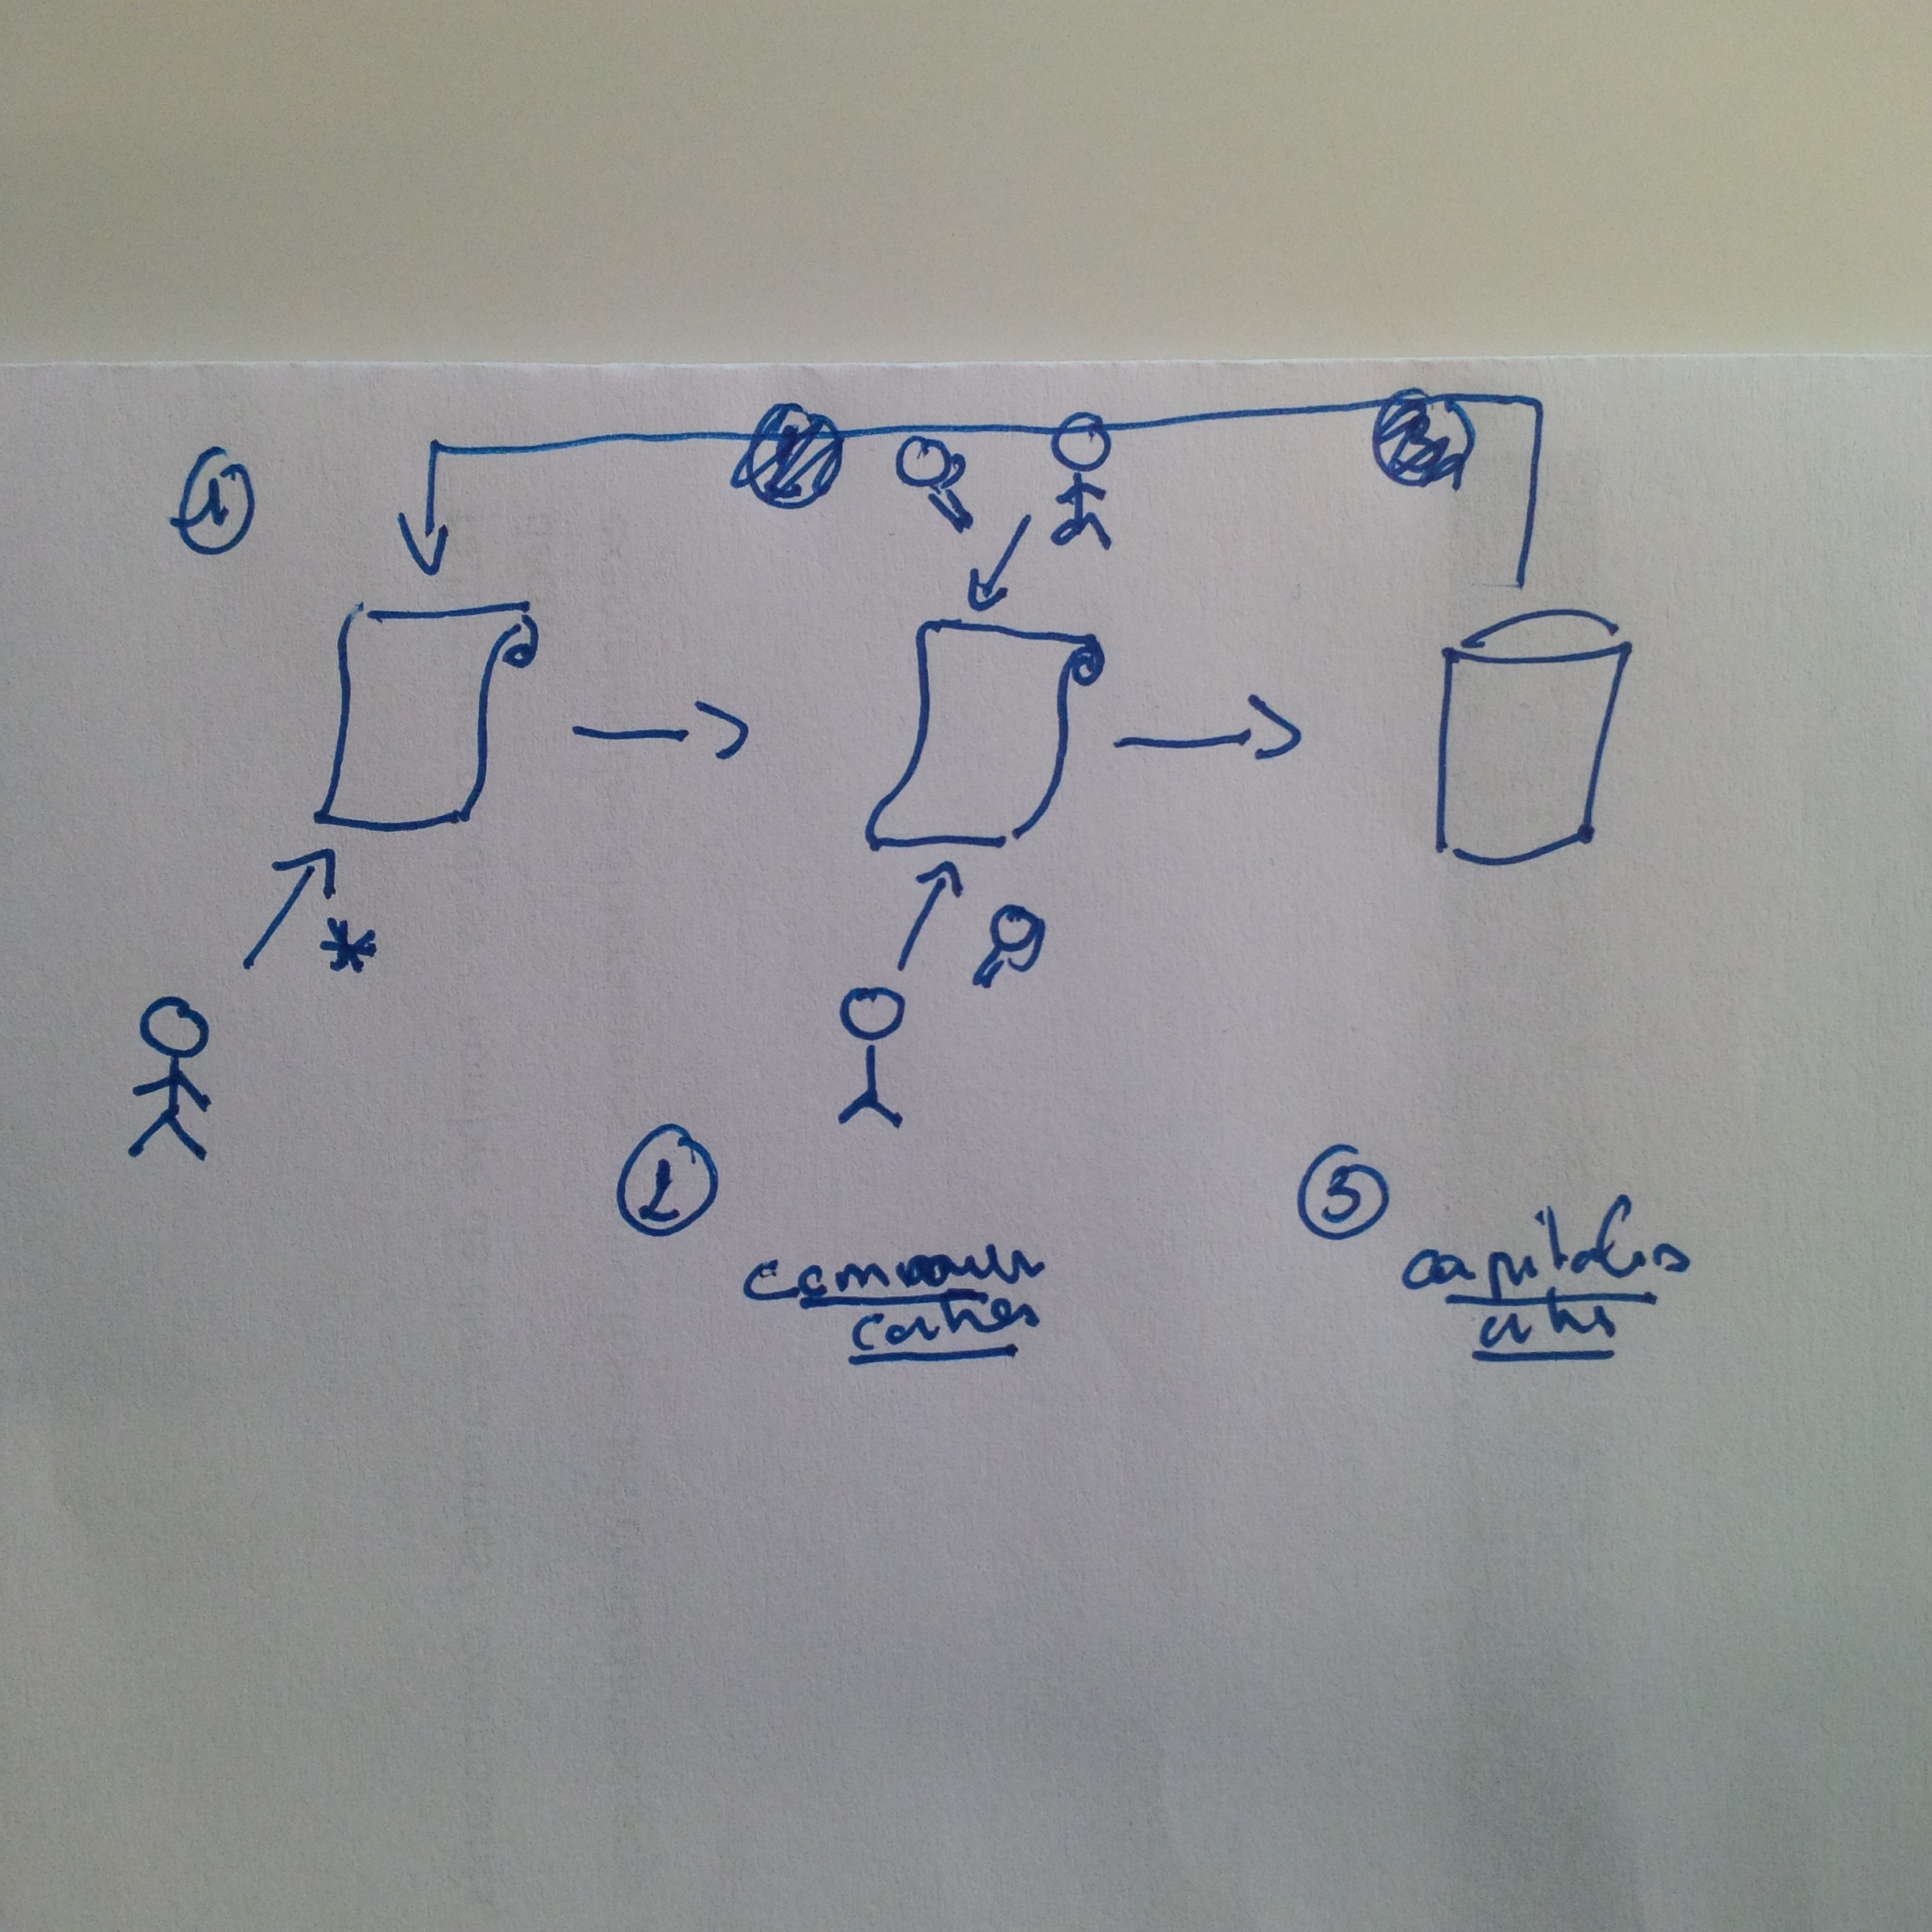
\includegraphics[width=10cm, height=3cm]{imgs/slide_application_patron}
\def\bonhomme#1{
\node[draw,circle,minimum width=3mm] (tete#1) {};
\coordinate (cou#1) at ([yshift=-2mm]tete#1.south);
\coordinate (entrejambes#1) at ([yshift=-2mm]cou#1);
\coordinate (main-gauche#1) at ([xshift=-3mm]cou#1);
\coordinate (main-droite#1) at ([xshift=3mm]cou#1);
\coordinate (pied-gauche#1) at ([xshift=-3mm,yshift=-3mm]entrejambes#1);
\coordinate (pied-droit#1) at ([xshift=3mm,yshift=-3mm]entrejambes#1);
\draw (tete#1.south) -- (entrejambes#1);
\draw (main-gauche#1) -- (main-droite#1);
\draw (pied-gauche#1) -- (entrejambes#1) -- (pied-droit#1);
}
\begin{tikzpicture}
    \begin{scope}[line width=2pt,every node/.style={line width=2pt}]
        \bonhomme{1}
        \begin{scope}[xshift=4cm]
            \bonhomme{2}
            \begin{scope}[xshift=1.5cm,yshift=3.5cm]
                \bonhomme{3}
            \end{scope}
        \end{scope}
    \end{scope}
    \foreach \i in {1,2,3} {
        \node[fit=(tete\i)(cou\i)(entrejambes\i)(main-gauche\i)(main-droite\i)(pied-gauche\i)(pied-droit\i),inner sep=0pt] (b\i) {};
    }
    \begin{scope}[every node/.style={line width=2pt,draw=black,rectangle,minimum height=12mm,minimum width=8.4mm,outer sep=2mm}]
        \foreach \i in {1,2} {
            \node (r\i) at ([xshift=1.5cm,yshift=1cm]tete\i.center) {};
        }
        \node[cylinder,shape border rotate=90] (bd) at ([xshift=4cm]r2.center) {};
    \end{scope}
    \begin{scope}[line width=2pt,->]
        \draw (b1) -- (r1) node[pos=.5,below right,inner sep=0pt] {*};
        \draw (b2) -- (r2) node[pos=.5,below right,magnifying glass,draw,outer sep=2mm] {};
        \draw (b3) -- (r2) node[pos=.5,right,outer sep=1mm,magnifying glass,draw] {};
        \draw (r1) -- (r2);
        \draw (r2) -- (bd);
        \draw (bd.north) |- ([yshift=1mm]tete3.north) coordinate[name=f] -| (r1.north);
    \end{scope}
    \begin{scope}[every node/.style={draw=black,circle,font=\footnotesize,outer sep=1mm,inner sep=1pt}]
        \node[above left] at (r1.north west) {1};
        \node[below] (t2) at (r2.south) {2};
        \node (t3) at (bd.south |- t2) {3};
    \end{scope}
    \node[below] at (t2.south) {communication};
    \node[below] at (t3.south) {capitalisation};
\end{tikzpicture}
\end{figure}
\begin{block}{}
Les \textbf{patrons de reconfiguration dynamique} documentent des solutions de
reconfiguration dynamique à des problèmes de conception récurrents.
\end{block}
%\begin{exampleblock}{}
%\begin{itemize}
%\item Programmation orientée objet : \textit{Design Patterns: Elements of
%Reusable Object-Oriented Software} 
%\item Architecture des systèmes distribués : \textit{Architecture,
%volume 4: A Pattern Language for Distributed Computing}
%\end{itemize}
%\end{exampleblock}
\end{frame}

%\begin{frame}{Problèmes rencontrés : modélisation de configuration}
%\begin{figure}
%\centering
%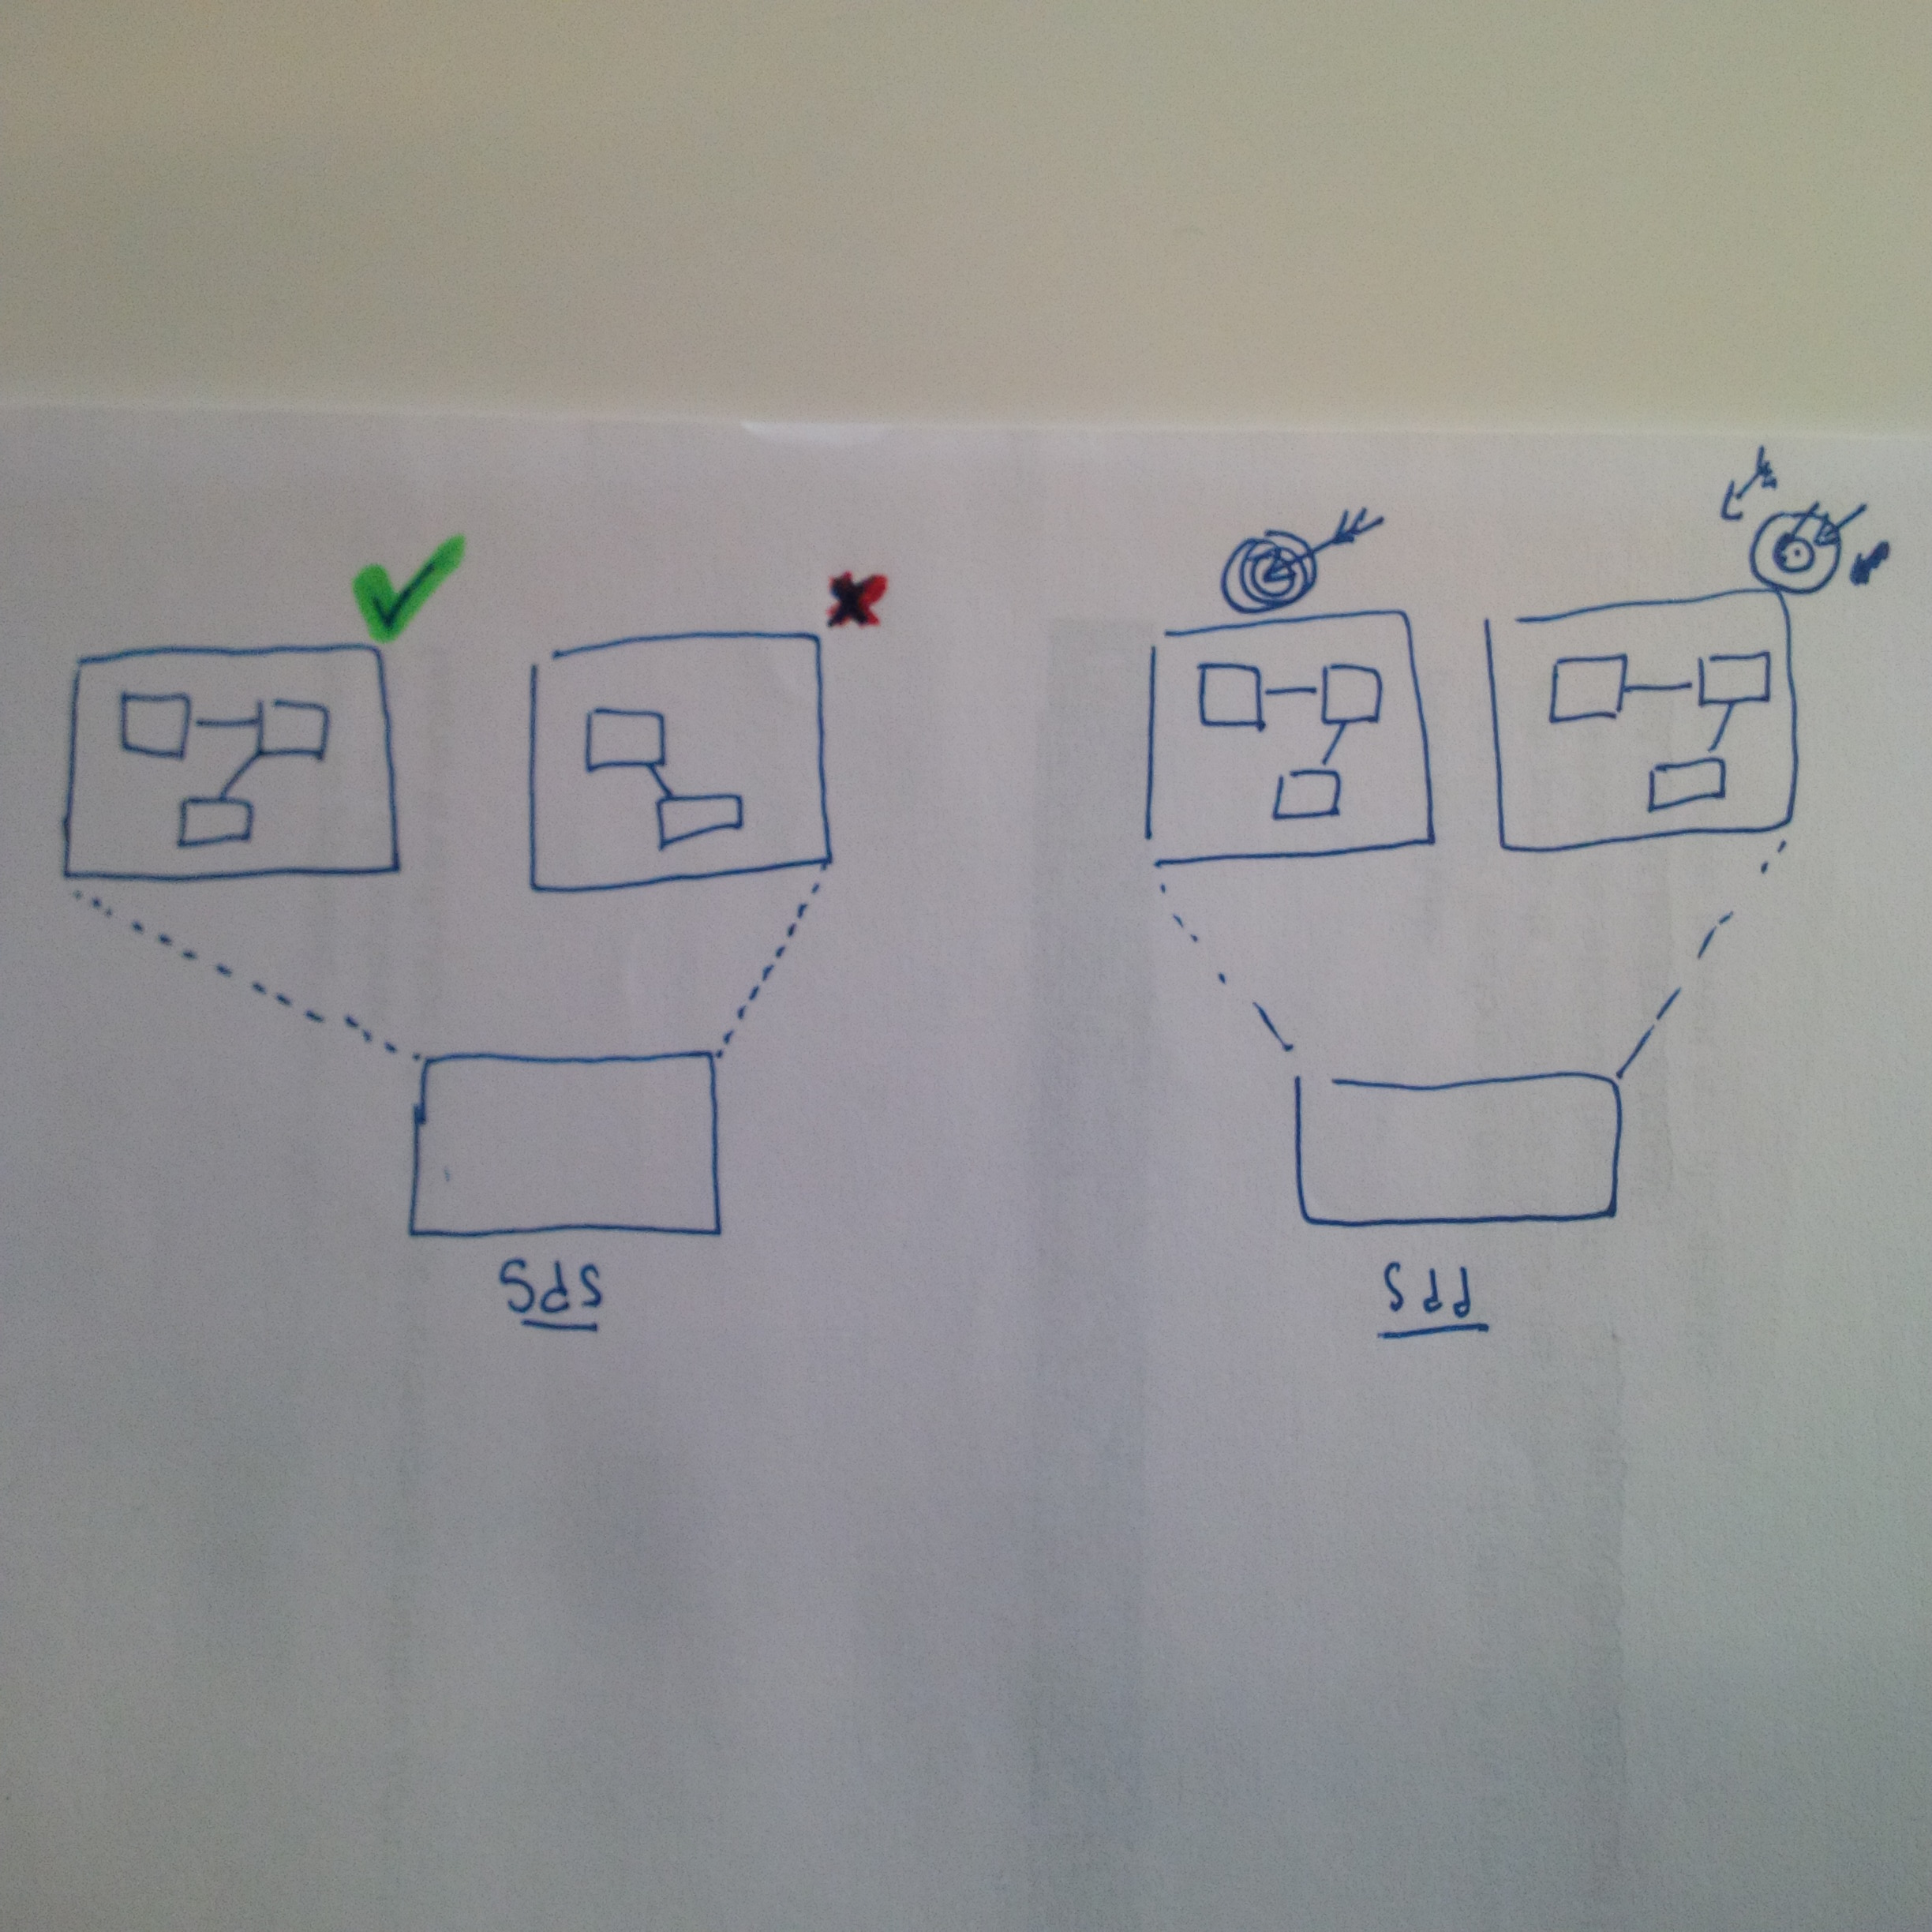
\includegraphics[width=10cm, height=4cm]{imgs/slide_probleme_modelisation.jpg}
%\end{figure} 
%\begin{definition}{}
%Un modèle est \textbf{exact} si il est
%factuel ou ne dévie pas trop du fait qu’il modélis
%\end{definition}
%\begin{definition}{}
%Un modèle est \textbf{précis} si il est suffisamment détaillé pour
%répondre au besoin de spécification, d'analyse ou de vérification.
%\end{definition}
%\end{frame}

%\begin{frame}{Problèmes recontrés : processus de reconfiguration}
%\begin{figure}
%\centering
%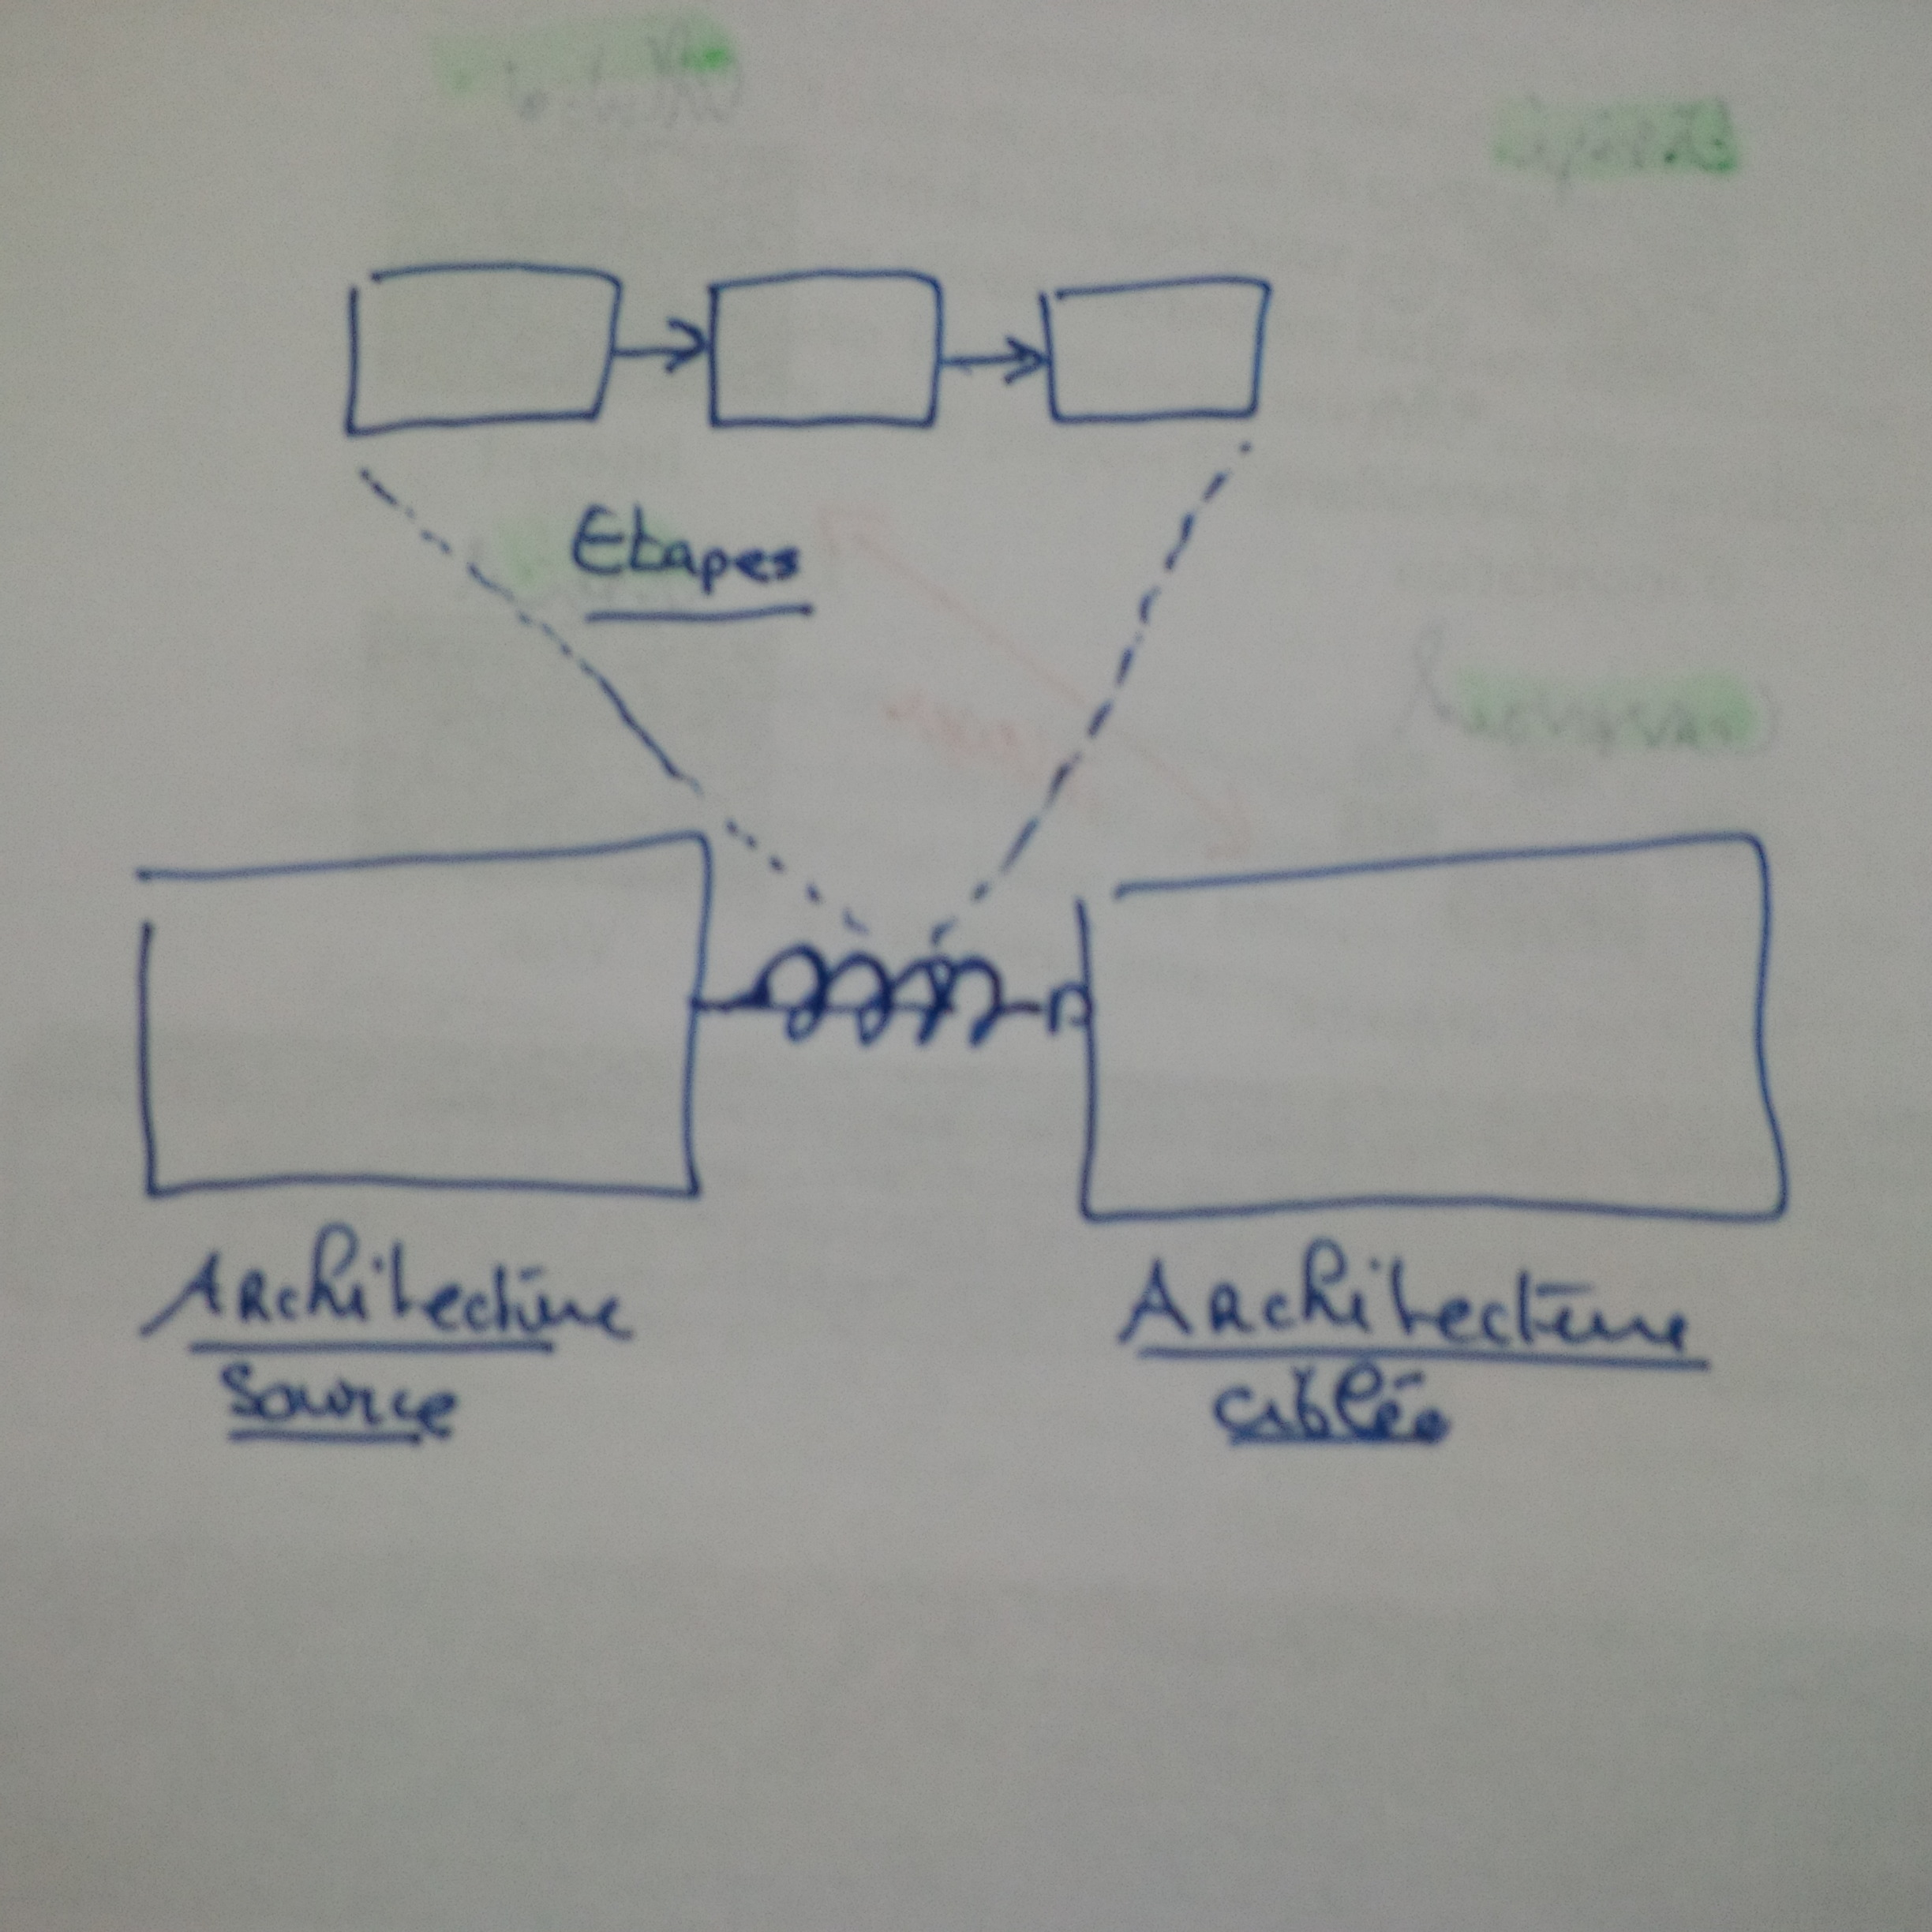
\includegraphics[width=\textwidth, height=0.6\textwidth]{imgs/slide_introduction_process.jpg}
%\end{figure}
%\end{frame}

\begin{frame}{Questions de recherche}
Comment l’architecte doit-il procéder pour faire évoluer un système de systèmes après son déploiement, dans le cadre du développement évolutionnaire ?\\
\begin{itemize}
    \item[Q1] Comment l’architecte modélise-t-il la configuration du système avec le niveau de précision et d’exactitude requis ?
    \item[Q2] Comment l’architecte peut-il documenter ses choix de conception d’une reconfiguration ?
    \item[Q3] Quel processus d’ingénierie l’architecte doit-il suivre pour concevoir la reconfiguration d’évolution du système de systèmes ?
\end{itemize}
\end{frame}

\begin{frame}{Plan de la soutenance}
\tableofcontents
\end{frame}

